This project was written as the Bachelor project by group SW606F13 - Software students from the Department of Computer Science at Aalborg University in the spring of 2013. The report documents the GIRAF project of 2013 and the implementation of the Train application. The application is developed for the Android platform. The reader is expected to be familiar with Java and UML. We have included our knowledge from all our previous semesters.
\\\\
When reading the report, there are a few things the reader should be aware of:
\begin{itemize}
\item When a reference to a source of a section or paragraph is given, the number of the source is written inside square brackets $[\;]$. The number is a reference to the bibliography list on page \pageref{chap:bib}.
\item When "we/us/our" is mentioned in the report, it is a referral to the authors of the report
\item In class diagrams a minus denotes a private attribute/method, and a plus denotes a public attribute/method. Italic class names are abstract classes.
\end{itemize}
\begin{center}
\includegraphics[page=4,width=0.7\linewidth]{img/opengl.pdf}
\end{center}
We would like to thank our supervisor Ulrik Mathias Nyman for the feedback he has given throughout the project.
